\begin{figure}[h!]
    \centering
    
    \begin{subfigure}[t]{0.48\textwidth}
        \begin{subfigure}[t]{\textwidth}
            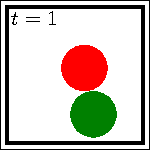
\includegraphics[width=0.22\textwidth]{figures/BBNF/BBNF3_cluster_2019_10_03_11_38_39/frame_00001.pdf}%
            ~
            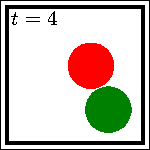
\includegraphics[width=0.22\textwidth]{figures/BBNF/BBNF3_cluster_2019_10_03_11_38_39/frame_00004.pdf}%
            ~
            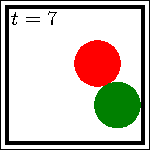
\includegraphics[width=0.22\textwidth]{figures/BBNF/BBNF3_cluster_2019_10_03_11_38_39/frame_00007.pdf}%
            ~
            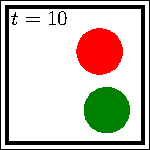
\includegraphics[width=0.22\textwidth]{figures/BBNF/BBNF3_cluster_2019_10_03_11_38_39/frame_00010.pdf}%
            % \vspace*{-0.2cm}
        \end{subfigure}
        \vspace*{-0.5cm}
        \caption{}
        \label{fig:balls:trajectory}
    \end{subfigure}%
    
    % \vspace*{-0.1cm}
    \begin{subfigure}[t]{0.48\textwidth}
        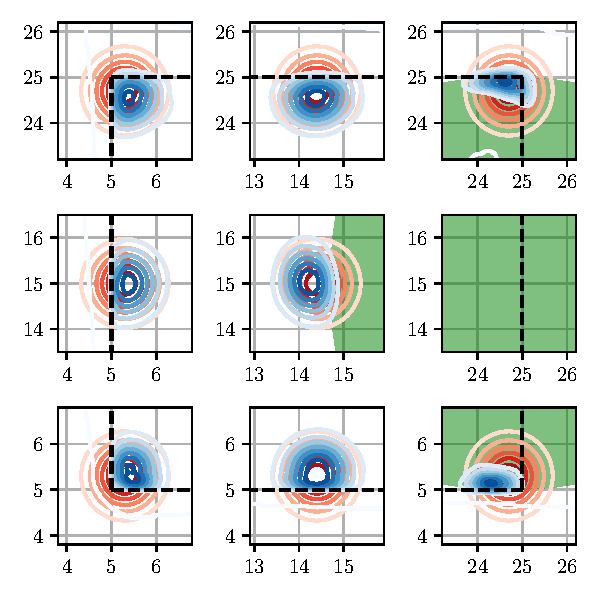
\includegraphics[width=\textwidth]{figures/BBNF/BBNF3_cluster_2019_10_03_11_38_39/BBNF3_density_array_2balls_00_000000.pdf}
        \vspace*{-0.7cm}
        \caption{}
        \label{fig:balls:space}
    \end{subfigure}%
    
    \vspace*{0.1cm}
    \begin{subfigure}[t]{0.45\textwidth}
        \begin{overpic}[width=\textwidth]{figures/BBNF/BBNF3_cluster_2019_10_03_11_38_39/bot_rate.pdf}
        \put (4, 4) {$p$}
        \put (44, 4) {$q_{\phi}$}
        \end{overpic}
        \vspace*{-0.5cm}
        \caption{}
        \label{fig:balls:rr}
    \end{subfigure}%
    \vspace*{-0.2cm}
    \caption{Results of the bouncing balls experiment introduced in Section \ref{sec:experiments:bb}, with two radius five, unit mass balls in an enclosure of size $30$.
    \ref{fig:balls:trajectory} shows an example trajectory of the system.
    \ref{fig:balls:space} shows, in red, the proposal distribution over the perturbation to the position of the first ball specified in the model, and the learned proposal in blue. The edge of the permissible region of the enclosure is shown as a black dashed line. The second ball is fixed at $\left[ 25, 15\right]$, and the induced invalid region shaded green. The flow has learned to deflect away from the disallowed regions.
    \ref{fig:balls:rr} shows the rejection rate as a function of the position of the first ball, with the second ball in the position shown. The trained proposal (right) has all but eliminated rejection in the permissible space compared to the a-priori specified proposal (left).
    The rejection rate under $p$ is high in the interior as the second ball may also leave the enclosure, whereas $q_{\phi}$ has practically eliminated rejection by \emph{jointly} proposing perturbations.}
    \label{fig:balls}
\end{figure}